\subsection{One-Way Layouts and the $F$ Test}

Analysis of variance compares several mean levels by splitting total variation into variation within treatment groups and variation between treatment groups.  The method is a multisample continuation of the equal-variance two-sample procedure, with design and randomisation assumptions kept explicit.

\begin{definition} \label{def:balanced-one-way-layout} \hlt{Balanced One-Way Layout}\\
For $I,J\in\N$, one factor has levels $i=1,\ldots,I$, each with exactly $J$ independent replicates $Y_{ij}$, $j=1,\ldots,J$.\\
The normal fixed-effects model satisfies $Y_{ij}=\mu+\alpha_i+\varepsilon_{ij}$, $\sum\limits_{i=1}^{I}\alpha_i=0$, and independent errors $\varepsilon_{ij}\sim N(0,\sigma^2)$.\\
\hlt{Structural Commentary}: $\mathbb{E}Y_{ij}=\mu+\alpha_i$, and $\sum\limits_{i=1}^{I}\alpha_i=0$ identifies $\mu$ as the average treatment mean.\\
\hlt{Key Insight}: $H_0:\alpha_i=0\ \forall i$ iff all treatment means are equal.
\end{definition}

\begin{definition} \label{def:one-way-anova-sums-of-squares} \hlt{One-Way Sums of Squares}\\
For a balanced one-way layout, set $\overline{Y}_{i\cdot}\defeq \frac1J\sum\limits_{j=1}^{J}Y_{ij}$ and $\overline{Y}_{\cdot\cdot}\defeq \frac{1}{IJ}\sum\limits_{i=1}^{I}\sum\limits_{j=1}^{J}Y_{ij}$.
\begin{enumerate}[label=(\roman*)]
\setlength{\itemsep}{0pt}
\item \hlt{Total}: $SS_{\mathrm{tot}}\defeq \sum\limits_{i=1}^{I}\sum\limits_{j=1}^{J}(Y_{ij}-\overline{Y}_{\cdot\cdot})^2$; grand-mean dispersion.
\item \hlt{Within-treatment}: $SS_W\defeq \sum\limits_{i=1}^{I}\sum\limits_{j=1}^{J}(Y_{ij}-\overline{Y}_{i\cdot})^2$; residual dispersion within treatments.
\item \hlt{Between-treatment}: $SS_B\defeq J\sum\limits_{i=1}^{I}(\overline{Y}_{i\cdot}-\overline{Y}_{\cdot\cdot})^2$; treatment-mean dispersion scaled by $J$.
\end{enumerate}
\hlt{Key Insight}: $SS_{\mathrm{tot}}=SS_W+SS_B$ separates within-treatment noise from between-treatment mean differences.
\end{definition}

\begin{proposition} \label{prop:one-way-sums-of-squares-decomposition} \hlt{One-Way Sum-of-Squares Decomposition}\\
For $I,J\in\N$ and observations $Y_{ij}$, set $\overline{Y}_{i\cdot}\defeq \frac{1}{J}\sum\limits_jY_{ij}$, $\overline{Y}_{\cdot\cdot}\defeq \frac{1}{IJ}\sum\limits_i\sum\limits_jY_{ij}$,\\
$SS_{\mathrm{tot}}\defeq\sum\limits_i\sum\limits_j(Y_{ij}-\overline{Y}_{\cdot\cdot})^2$, $SS_W\defeq\sum\limits_i\sum\limits_j(Y_{ij}-\overline{Y}_{i\cdot})^2$, and $SS_B\defeq J\sum\limits_i(\overline{Y}_{i\cdot}-\overline{Y}_{\cdot\cdot})^2$. Then $SS_{\mathrm{tot}}=SS_W+SS_B$.
\begin{proof}
Set $r_{ij}\defeq Y_{ij}-\overline{Y}_{i\cdot}$ and $b_i\defeq \overline{Y}_{i\cdot}-\overline{Y}_{\cdot\cdot}$. Then $Y_{ij}-\overline{Y}_{\cdot\cdot}=r_{ij}+b_i$ and $\sum\limits_jr_{ij}=0\ \forall i$.\\
Thus $SS_{\mathrm{tot}}=\sum\limits_i\sum\limits_j(r_{ij}+b_i)^2=\sum\limits_i\sum\limits_jr_{ij}^2+2\sum\limits_i b_i\sum\limits_jr_{ij}+J\sum\limits_i b_i^2=SS_W+SS_B$.\\
\hlt{Structural Commentary}: $Y_{ij}-\overline{Y}_{\cdot\cdot}=r_{ij}+b_i$, where $r_{ij}\defeq Y_{ij}-\overline{Y}_{i\cdot}$ and $b_i\defeq\overline{Y}_{i\cdot}-\overline{Y}_{\cdot\cdot}$.\\
\hlt{Key Insight}: $\sum\limits_jr_{ij}=0\ \forall i$ annihilates the cross term $2\sum\limits_i b_i\sum\limits_jr_{ij}$.
\end{proof}
\end{proposition}

\begin{figure}[H]
  \centering
  % Source: supplied Chapter 12 screenshots on one-way analysis of variance.
% Schematic redraw, not a reproduction of the scanned figures.
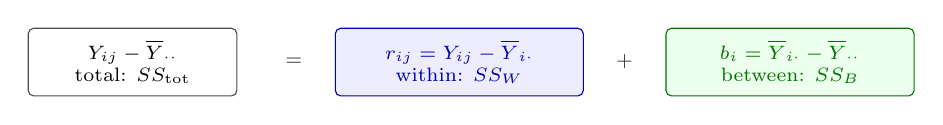
\begin{tikzpicture}[
  x=1cm,
  y=1cm,
  every node/.style={font=\scriptsize},
  line cap=round,
  line join=round,
  total/.style={draw=black!70, rounded corners=2pt, align=center,
    minimum width=2.65cm, minimum height=0.86cm, inner xsep=5pt, inner ysep=3pt},
  within/.style={draw=blue!70!black, text=blue!70!black, fill=blue!7,
    rounded corners=2pt, align=center, minimum width=3.15cm, minimum height=0.86cm,
    inner xsep=5pt, inner ysep=3pt},
  between/.style={draw=green!45!black, text=green!45!black, fill=green!7,
    rounded corners=2pt, align=center, minimum width=3.15cm, minimum height=0.86cm,
    inner xsep=5pt, inner ysep=3pt},
  formula/.style={align=center, text=black!78}
]
  \node[total] (total) at (-3.8,0)
    {$Y_{ij}-\overline{Y}_{\cdot\cdot}$\\total: $SS_{\mathrm{tot}}$};
  \node[formula] at (-1.75,0) {$=$};
  \node[within] (within) at (0.35,0)
    {$r_{ij}=Y_{ij}-\overline{Y}_{i\cdot}$\\within: $SS_W$};
  \node[formula] at (2.45,0) {$+$};
  \node[between] (between) at (4.55,0)
    {$b_i=\overline{Y}_{i\cdot}-\overline{Y}_{\cdot\cdot}$\\between: $SS_B$};
\end{tikzpicture}

  \caption{Squaring and summing gives $SS_{\mathrm{tot}}=SS_W+SS_B$; large $MS_B/MS_W$ suggests treatment effects.}
  \label{fig:anova-sums-of-squares-decomposition}
\end{figure}

\begin{lemma} \label{lem:mean-centering-expected-square} \hlt{Expected Squared Deviation from a Sample Mean}\\
Let $X_1,\ldots,X_n$ be independent with $\mathbb{E}X_i=\mu_i$ and $\operatorname{Var}(X_i)=\sigma^2$ for $1\leq i\leq n$.\\
Set $\overline{X}\defeq \frac{1}{n}\sum\limits_{i=1}^{n}X_i$ and $\overline{\mu}\defeq \frac{1}{n}\sum\limits_{i=1}^{n}\mu_i$.
Then $\mathbb{E}(X_i-\overline{X})^2=(\mu_i-\overline{\mu})^2+\frac{n-1}{n}\sigma^2$ for $1\leq i\leq n$.
\begin{proof}
Set $U_i\defeq X_i-\overline{X}$. Then $\mathbb{E}U_i=\mu_i-\overline{\mu}$, $\operatorname{Var}(\overline{X})=\frac{\sigma^2}{n}$, and $\operatorname{Cov}(X_i,\overline{X})=\frac{\sigma^2}{n}$ by independence.\\
Hence $\operatorname{Var}(U_i)=\operatorname{Var}(X_i)+\operatorname{Var}(\overline{X})-2\operatorname{Cov}(X_i,\overline{X})=\sigma^2+\frac{\sigma^2}{n}-2\frac{\sigma^2}{n}=\frac{n-1}{n}\sigma^2$.\\
Thus $\mathbb{E}U_i^2=(\mathbb{E}U_i)^2+\operatorname{Var}(U_i)=(\mu_i-\overline{\mu})^2+\frac{n-1}{n}\sigma^2$.\\
\hlt{Structural Commentary}: $X_i-\overline{X}$ has mean $\mu_i-\overline{\mu}$ and variance $\operatorname{Var}(X_i-\overline{X})=\frac{n-1}{n}\sigma^2$.\\
\hlt{Key Insight}: $\operatorname{Cov}(X_i,\overline{X})=\frac{\sigma^2}{n}$ removes exactly one $\frac{\sigma^2}{n}$ from the raw variance $\sigma^2$.
\end{proof}
\end{lemma}

\begin{theorem} \label{thm:one-way-anova-expected-mean-squares} \hlt{Expected One-Way Sums of Squares}\\
For $I,J\in\N$, let $Y_{ij}=\mu+\alpha_i+\varepsilon_{ij}$, $1\leq i\leq I$, $1\leq j\leq J$, with $\sum\limits_i\alpha_i=0$, independent errors satisfying\\
$\mathbb{E}\varepsilon_{ij}=0$, $\operatorname{Var}(\varepsilon_{ij})=\sigma^2$. Set $\overline{Y}_{i\cdot}\defeq \frac{1}{J}\sum\limits_jY_{ij}$, $\overline{Y}_{\cdot\cdot}\defeq \frac{1}{IJ}\sum\limits_i\sum\limits_jY_{ij}$.\\
Then $SS_W\defeq\sum\limits_i\sum\limits_j(Y_{ij}-\overline{Y}_{i\cdot})^2$, $SS_B\defeq J\sum\limits_i(\overline{Y}_{i\cdot}-\overline{Y}_{\cdot\cdot})^2$; $\mathbb{E}(SS_W)=I(J-1)\sigma^2$\\
and $\mathbb{E}(SS_B)=(I-1)\sigma^2+J\sum\limits_i\alpha_i^2$. Hence $S_p^2\defeq \frac{SS_W}{I(J-1)}$ satisfies $\mathbb{E}S_p^2=\sigma^2$.\\
\begin{proof} For fixed $i$, Lemma \ref{lem:mean-centering-expected-square} with $\mu_{ij}=\mu+\alpha_i$ gives $\mathbb{E}\sum\limits_j(Y_{ij}-\overline{Y}_{i\cdot})^2=(J-1)\sigma^2$, hence $\mathbb{E}SS_W=I(J-1)\sigma^2$.\\
For $\overline{Y}_{i\cdot}$, $\mathbb{E}\overline{Y}_{i\cdot}=\mu+\alpha_i$, $\operatorname{Var}(\overline{Y}_{i\cdot})=\frac{\sigma^2}{J}$, and $\frac{1}{I}\sum\limits_i(\mu+\alpha_i)=\mu$. By Lemma \ref{lem:mean-centering-expected-square}, $(\overline{Y}_{i\cdot})_{i=1}^{I}$ gives\\
$\mathbb{E}\sum\limits_i(\overline{Y}_{i\cdot}-\overline{Y}_{\cdot\cdot})^2=\sum\limits_i\alpha_i^2+\frac{I-1}{J}\sigma^2$, so $\mathbb{E}SS_B=J\sum\limits_i\alpha_i^2+(I-1)\sigma^2$. Thus $\mathbb{E}S_p^2=\frac{\mathbb{E}SS_W}{I(J-1)}=\sigma^2$.\\
\hlt{Structural Commentary}: $\mathbb{E}SS_W$ depends only on $\sigma^2$; $\mathbb{E}SS_B$ adds $J\sum\limits_i\alpha_i^2$.\\
\hlt{Key Insight}: Under $\alpha_i=0\ \forall i$, $\mathbb{E}\{\frac{SS_B}{I-1}\}=\mathbb{E}\{\frac{SS_W}{I(J-1)}\}=\sigma^2$.
\end{proof}
\end{theorem}

\begin{theorem} \label{thm:one-way-anova-f-test} \hlt{Normal-Theory One-Way $F$ Test}\\
For $I,J\in\N$, let $Y_{ij}=\mu+\alpha_i+\varepsilon_{ij}$, $1\leq i\leq I$, $1\leq j\leq J$, with $\sum\limits_i\alpha_i=0$ and independent errors $\varepsilon_{ij}\sim N(0,\sigma^2)$.\\
Set $\overline{Y}_{i\cdot}\defeq \frac{1}{J}\sum\limits_jY_{ij}$, $\overline{Y}_{\cdot\cdot}\defeq \frac{1}{IJ}\sum\limits_i\sum\limits_jY_{ij}$, $SS_W\defeq\sum\limits_i\sum\limits_j(Y_{ij}-\overline{Y}_{i\cdot})^2$, $SS_B\defeq J\sum\limits_i(\overline{Y}_{i\cdot}-\overline{Y}_{\cdot\cdot})^2$.\\
$MS_W\defeq \frac{SS_W}{I(J-1)}$, $MS_B\defeq \frac{SS_B}{I-1}$; $\frac{SS_W}{\sigma^2}\sim \chi^2_{I(J-1)}$; if $H_0:\alpha_i=0\ \forall i$, then $\frac{SS_B}{\sigma^2}\sim \chi^2_{I-1}$, $SS_B\perp\!\!\!\perp SS_W$, $F\defeq \frac{MS_B}{MS_W}\sim F_{I-1,I(J-1)}$.
\begin{proof} Let $C_m\defeq \mathrm{Id}_m-m^{-1}\mathbf{1}_m\mathbf{1}_m^\top$, so $C_m^2=C_m=C_m^\top$ and $\operatorname{rank}C_m=m-1$.\\
For each $i$, $Z_i\defeq\frac{1}{\sigma}(Y_{i1}-\mu-\alpha_i,\ldots,Y_{iJ}-\mu-\alpha_i)^\top\sim N_J(0,\mathrm{Id}_J)$ independently,\\
$\frac{1}{\sigma^2}\sum\limits_j(Y_{ij}-\overline{Y}_{i\cdot})^2=Z_i^\top C_JZ_i\sim\chi^2_{J-1}$. Summing over independent treatments gives $\frac{SS_W}{\sigma^2}\sim\chi^2_{I(J-1)}$.\\
Under $H_0$, $\widetilde{Z}\defeq \sqrt{J}\sigma^{-1}(\overline{Y}_{1\cdot}-\mu,\ldots,\overline{Y}_{I\cdot}-\mu)^\top\sim N_I(0,\mathrm{Id}_I)$, and $\frac{SS_B}{\sigma^2}=\widetilde{Z}^\top C_I\widetilde{Z}\sim\chi^2_{I-1}$.\\
For each $i$, $C_JZ_i\perp\!\!\!\perp \mathbf{1}_J^\top Z_i$ by orthogonal normal components.\\
Hence $SS_W\perp\!\!\!\perp(\overline{Y}_{1\cdot},\ldots,\overline{Y}_{I\cdot})$ and $SS_W\perp\!\!\!\perp SS_B$. Thus $F=\frac{SS_B}{I-1}/\frac{SS_W}{I(J-1)}=\frac{MS_B}{MS_W}\sim F_{I-1,I(J-1)}$.\\
\hlt{Structural Commentary}: $IJ=1+I(J-1)+(I-1)$ partitions df into mean, residual, and contrast subspaces.\\
\hlt{Key Insight}: Under $H_0$, $MS_B$ and $MS_W$ are independent $\sigma^2$ estimators, so $\frac{MS_B}{MS_W}$ has an $F$ law.
\end{proof}
\end{theorem}

\begin{method} \label{meth:one-way-anova-unequal-sample-sizes} \hlt{Unequal Sample Sizes}\\
For $I\in\N$, treatment $i$ has observations $Y_{ij}$, $1\leq j\leq J_i$, with $J_i\in\N$ and $N\defeq\sum\limits_{i=1}^{I}J_i$.
\begin{enumerate}[label=(\roman*)]
\setlength{\itemsep}{0pt}
\item $\overline{Y}_{i\cdot}\defeq \frac{1}{J_i}\sum\limits_{j=1}^{J_i}Y_{ij}$ and $\overline{Y}_{\cdot\cdot}\defeq \frac{1}{N}\sum\limits_{i=1}^{I}\sum\limits_{j=1}^{J_i}Y_{ij}$.
\item $SS_W\defeq\sum\limits_{i=1}^{I}\sum\limits_{j=1}^{J_i}(Y_{ij}-\overline{Y}_{i\cdot})^2$, $SS_B\defeq\sum\limits_{i=1}^{I}J_i(\overline{Y}_{i\cdot}-\overline{Y}_{\cdot\cdot})^2$, $SS_{\mathrm{tot}}\defeq\sum\limits_{i=1}^{I}\sum\limits_{j=1}^{J_i}(Y_{ij}-\overline{Y}_{\cdot\cdot})^2$\\
satisfy $SS_{\mathrm{tot}}=SS_W+SS_B$.
\item $\operatorname{df}_W=N-I$ and $\operatorname{df}_B=I-1$.
\item If $Y_{ij}=\mu_i+\varepsilon_{ij}$ with independent $\varepsilon_{ij}\sim N(0,\sigma^2)$ and $H_0:\mu_1=\cdots=\mu_I$, then $F\defeq \frac{\frac{SS_B}{I-1}}{\frac{SS_W}{N-I}}\sim F_{I-1,N-I}$.
\end{enumerate}
\end{method}

\begin{example} \label{ex:tablet-laboratories-one-way-anova} \hlt{Generic Balanced One-Way ANOVA}\\
Let $I=7$, $J=10$, and $Y_{ij}=\mu_i+\varepsilon_{ij}$ with independent errors $\varepsilon_{ij}\sim N(0,\sigma^2)$. Suppose the ANOVA table is
\[
\begin{array}{c|rrrr}
\text{Component} & df & SS & MS & F\\ \hline
\text{Treatment} & 6 & .125 & .021 & 5.66\\
\text{Error} & 63 & .231 & .0037 & \\
\text{Total} & 69 & .356 & &
\end{array}
\]
Then $F=5.66$ has null law $F_{6,63}$, $p=\mathbb{P}(F_{6,63}\geq5.66)<.01$, and $H_0:\mu_1=\cdots=\mu_7$ is rejected at level $.01$.\\
If diagnostics are adequate, between-treatment variation exceeds within-treatment noise.
\end{example}

\begin{remark} \label{rem:one-way-anova-assumptions} \hlt{Assumptions and Robustness}\\
For $Y_{ij}=\mu_i+\varepsilon_{ij}$, the one-way $F$ calibration assumes independent $\varepsilon_{ij}\sim N(0,\sigma^2)$. Balance softens variance heterogeneity; clustered, paired, blocked, or repeated data require dependence modeling.
\end{remark}
